\chapter{Results}\label{ch:cfd}
\begin{em}
The Poisson binomial recursion describes the particle number distribution that connects the grand canonical ensemble to the canonical ensemble. To see if this method is accurate, it will be tested  against Sch\"onhammer's exact solution for the one dimensional linear energy spectrum. Once agreement is found, the theoretical results for the error in temperature measurement will be calculated. Specifically, linear and quadratic spectra with a nondegenerate, a filled degenerate, and a partially filled degenerate Fermi level will be compared to the theoretical models. Lastly, a special case where a spectrum has a Fermi level that is almost degenerate will be considered.  
\end{em}

\section{Benchmarking}
To check the method using the Poisson binomial recursion relation, the results can be benchmarked against a known solution. For this, we turn to Sch\"onhammer's solution for the 1D linear harmonic oscillator. This was previously considered in Section 1.5 and has an exact solution given by Eq.\@ (\ref{schoneqn}). Applying the Poisson binomial recursion, the results can be plotted on top of the exact solution as shown in Fig.\@ (\ref{fig: schon solution}). It is more useful to show the difference as seen in Fig.\@ (\ref{fig: schon diff}). 

There are two important parts of Fig.\@ (\ref{fig: schon diff}) that are worth noting. The first is the scale of the y-axis. This is the difference between the Sch\"onhammer's exact solution and the program solution. The range of $10^{-8}$ is important to note because this was the precision parameter that was set in the code. If a higher level of accuracy is required in this calculation, the precision can easily be changed.  

\begin{figure}[H]
    \centering
    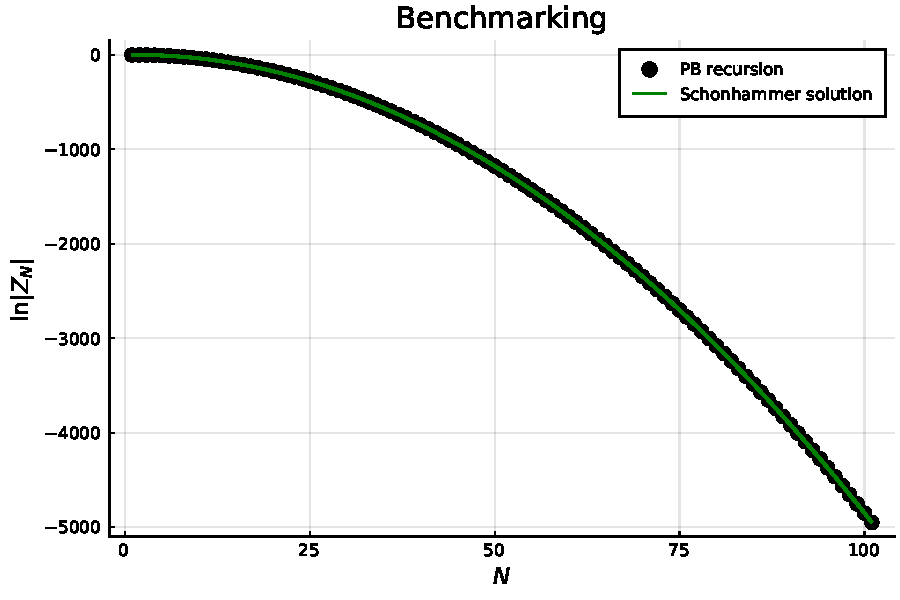
\includegraphics[scale=0.75]{figures/pdf/Benchmarking.pdf}
    \caption{Solution from Poisson Binomial recursive method versus the exact solution for the 1D simple harmonic oscillator. The black circles are the solutions from the Poisson Binomial recursion method. The green line is the exact solution using Sch\"onhammer's Eq.(\ref{schoneqn})}
    \label{fig: schon solution}
\end{figure}
\begin{figure}[H]
    \centering
    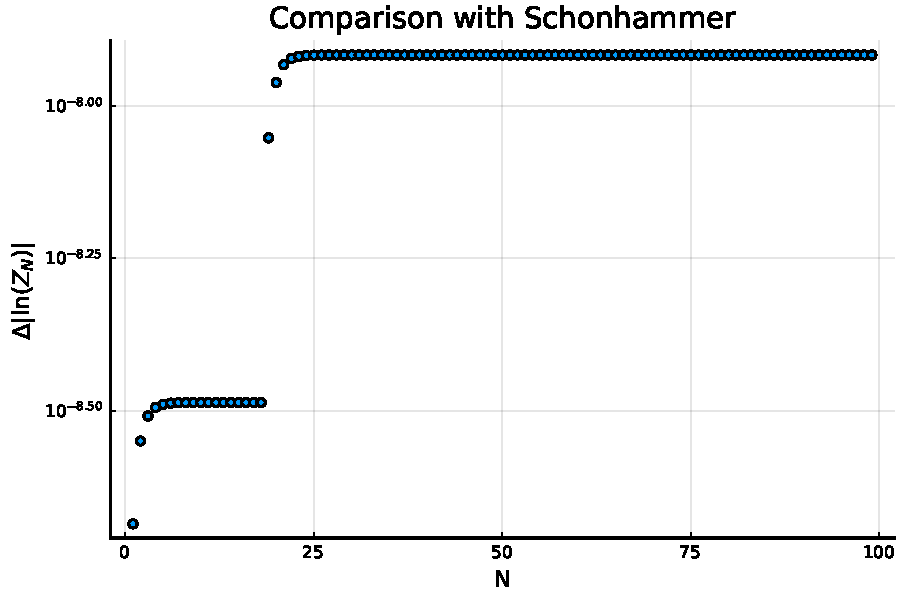
\includegraphics[scale=0.75]{figures/pdf/Benchdiff.pdf}
    \caption{The difference between the solutions presented in Fig. (\ref{fig: schon solution}). The precision of the Poisson binomial method was set to $10^{-8}$ which controls the range of the y-axis. The jump in error is due to the exclusion of terms below the Fermi level. Terms are chosen to be excluded if their occupation probability differs from one by a chosen cutoff value. In this case they are assumed to be in an occupied state. }
    \label{fig: schon diff}
\end{figure}

The other part to note is the jump in the error. This is due to the process of building the initial occupation probability distribution. As a reminder, the program is dealing with a fixed number of particles at ultra-low temperatures. At these temperatures, only the region around the Fermi level will have any sort of probability away from one or zero. Therefore, to increase the speed of the calculation, the states that are above a cutoff value are certain to be occupied. For these states with occupation probability of one, a counter keeps track of the number of particles and their probabilities are not included in the distribution. Similarly, any probability that is below the cutoff is not included because it is taken to have a zero probability of being occupied. This process saves memory and makes the calculations much faster. The downside to this process is that a small error is introduced. This is the source of the jump shown in Fig.\@ (\ref{fig: schon diff}). At this point, energy levels are left out of the distribution. Again, the error is controllable based on the precision chosen by the user.

\section{Controlling Chemical Potential}
The key role of the chemical potential is to ensure that the grand canonical ensemble has the correct number of particles in the system. The correct choice in chemical potential will affect the error of the measurement. Therefore, it's necessary to choose $\mu$ such that 
\begin{equation}
    \avg{N}=\sum_i \avg{p_i}
\end{equation}

where $N$ is the number of particles in the true canonical system. In the previous section, the partition function was calculated for different values of $N$. For each of these calculations, the choice in "fictitious" chemical potential is different. One interesting question is how much does this choice in chemical potential affect the error when calculating the partition function. To inspect this, we can set the chemical potential to a value and proceed with the same benchmarking code. The results of this are shown in Fig.\@ (\ref{fig:Errors}). We can see that the correct chemical potential will provide a minimum at its corresponding particle number value. After that, it increases as some absolute value of the distance from the correct $N$ value. Therefore, it is necessary that the chemical potential be updated each step in order to keep the errors at the minimum. 

\begin{figure}[H]
    \centering
    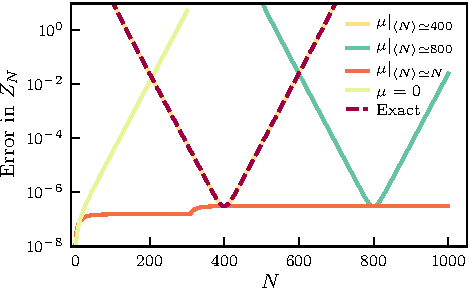
\includegraphics[scale=1.4]{figures/pdf/Plot1.pdf}
    \caption{The error associated with keeping the chemical potential $\mu$ fixed for a range of $N$ particles values. The accuracy of $\mu|_N$ is at the minimum error in a small range around $N$. The further $N$ is away from $\mu|_N$, the larger the error becomes. Therefore, it's necessary to recalculated $\mu$ for each value of $N$ in order to keep the error of the canonical partition function $Z_N$ to a minimum. This figure was provided by Jiangyong Yu. }
    \label{fig:Errors}
\end{figure}

\section{Numerical results of nondegenerate spectra}
In this section, we will consider the case where our spectrum is nondegenerate. From Section \ref{section:simpleexample}, we expect that the error of the temperature measurement $\beta^*$ in the grand canonical ensemble should reach $100\%$ once $\beta$ gets sufficiently large. We also saw the same result in Section \ref{section:filleddegen} when $g_0=g_1=g_{-1}=...=1$ in Eq.\@ (\ref{filldegencheck}). We consider the simple harmonic oscillator (linear spectrum) and the potential well spectrum (quadratic spectrum). The numerical results are shown in Figs.\@ (\ref{fig:linnondeg}) and (\ref{fig:quadnondeg}) where the y-axis is $\frac{\delta\beta}{\beta}=\frac{\beta^*-\beta}{\beta}$. %An interesting difference between the two figures is length of the x-axis.
The linear spectrum reaches $100\%$ error slower than the quadratic error. This is due to the spacing between energy levels. For the linear spectrum, this spacing is constant, while the quadratic spectrum has a spacing that linearly increases. This means that more energy is required to fill the first excited state for the quadratic spectrum as the number of particles increases. The spacing term $\Delta_0$ will always increase, and thus the Boltzmann probability $e^{-\beta\Delta_0}$ that the state is occupied will continually decrease. For this reason, it is more difficult to calculate the error for linear spectra. 

\begin{figure}[H]
    \centering
    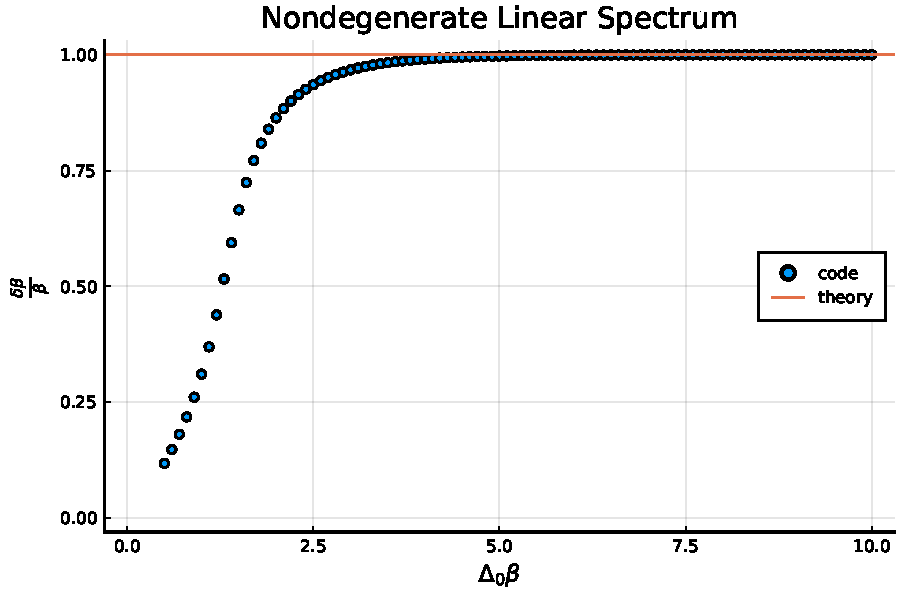
\includegraphics[scale=.75]{figures/pdf/linE_nondeg_N10.pdf}
    \caption{Error in $\beta^*$ measurement for a nondegenerate linear energy spectrum. Once $\Delta_0\beta$ is large enough, the error calculated from the code increases to $100\%$ as expected from the theory. }
    \label{fig:linnondeg}
\end{figure}

\begin{figure}[H]
    \centering
    \includegraphics[scale=0.75]{figures/pdf/quadE_nondeg_N10_Δ0=6.333.pdf}
    \caption{Error in $\beta^*$ measurement for a nondegenerate quadratic energy spectrum. Once $\Delta_0\beta$ is large enough, the error calculated from the code increases to $100\%$ as expected from the theory. }
    \label{fig:quadnondeg}
\end{figure}


\section{Numerical results of degenerate spectra}
In this section, we consider degenerate spectra. Specifically, we want to verify the equations in Section \ref{section:degenerate}. We first consider the case where the Fermi level is filled and then consider the case of partial filling. Finally, we investigate a special case where the Fermi level is almost degenerate. 
\subsection{Filled Fermi Level}
To start, the linear energy spectrum is used. Eq.\@ (\ref{filldegen}) is compared with the results from the recursion calculation Fig.\@ (\ref{fig:Filled}).  

\begin{figure}[H]
    \centering
    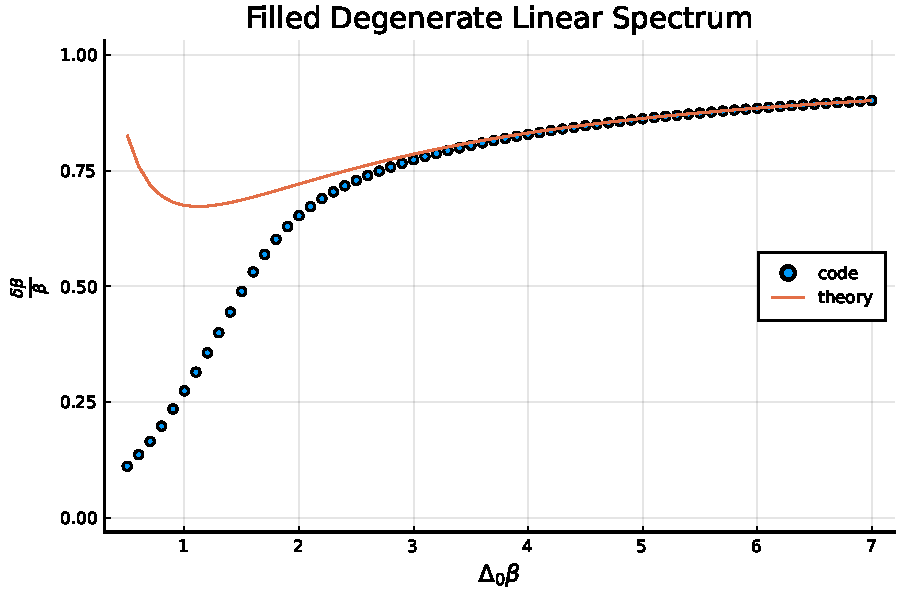
\includegraphics[scale=0.75]{figures/pdf/linE_filldegen_g0-2_N10.pdf}
    \caption{Error in $\beta^*$ measurement for a linear energy spectrum with a filled degenerate Fermi level. Once $\Delta_0\beta$ is large enough, the error calculated from the code follows the theoretical line in orange.}
    \label{fig:Filled}
\end{figure}

We can see that the error follows the theory once $\beta$ is sufficiently large. To further inspect this, consider rewriting Eq.\@ (\ref{filldegen}) in the following way. 
\begin{align}
    \frac{\delta\beta}{\beta}&=1-\frac{\ln(g_0g_1)}{\Delta_0\beta}\nonumber\\
    \frac{\delta\beta}{\beta}-1&=-\frac{\ln(g_0g_1)}{\Delta_0\beta}\nonumber\\
    \beta\Delta_0-\delta\beta\Delta_0&=\ln(g_0g_1) \label{3.2}
\end{align}
In this calculation, I have neglected the exponential term for convenience. Eq.\@ (\ref{3.2}) is then plotted against the program as shown in Fig. (\ref{fig:FilledDegenerateLinearSpectrumAdjustedError}). 
\begin{figure}[H]
    \centering
    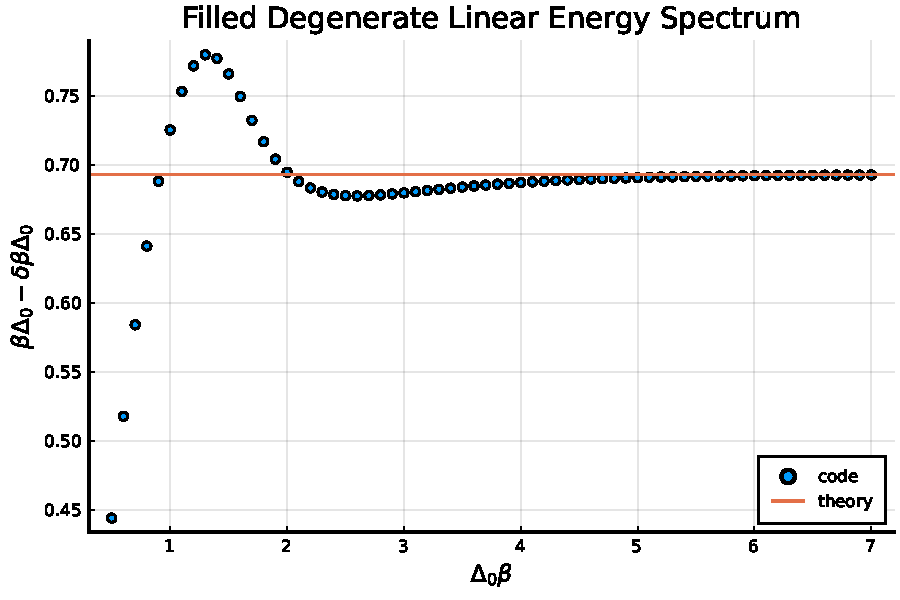
\includegraphics[scale=0.75]{figures/pdf/linE_filldegen_g0-2_N10_1.pdf}
    \caption{Error in $\beta^*$ measurement for a linear energy spectrum with a filled
degenerate Fermi level. The figure is adjusted to plot Eq.\@ (\ref{3.2}). Once $\Delta_0\beta$ is large enough, the $\ln(g_0g_1)$ limit is reached. For the case shown above, $g_0=2$ and $g_1=1$ so the asymptotic limit is $\ln(2)$ as shown in orange.}
    \label{fig:FilledDegenerateLinearSpectrumAdjustedError}
\end{figure}
Again, we can see that at high enough $\beta$ the program aligns with the theory. 

Now I will consider the filled degenerate quadratic energy spectrum. The analysis will be the same, so Eq.\@ (\ref{3.2}) will still be used. The results of the program are shown in Figs.\@ (\ref{fig:FilledDegenerate}) and (\ref{fig:FilledDegenerate2}). 

\begin{figure}[H]
    \centering
    \includegraphics[scale=0.75]{figures/pdf/quadE_filldegen_g0-2_N10_Δ0-7.pdf}
    \caption{Error in $\beta^*$ measurement for a quadratic energy spectrum with a filled
degenerate Fermi level. Once the temperature is small enough, the error calculated from the code
follows the theoretical line in orange.}
    \label{fig:FilledDegenerate}
\end{figure}

\begin{figure}[H]
    \centering
    \includegraphics[scale=0.75]{figures/pdf/quadE_filldegen_g0-2_N10_Δ0-7_1.pdf}
    \caption{Error in $\beta^*$ measurement for a quadratic energy spectrum with a filled
degenerate Fermi level. The figure is adjusted to plot Eq.\@ (\ref{3.2}). Once $\Delta_0\beta$ is large enough, the $\ln(g_0g_1)$ limit is reached. For the case shown above, $g_0=2$ and $g_1=1$ so the asymptotic limit is $\ln(2)$ as shown in orange.}
    \label{fig:FilledDegenerate2}
\end{figure}
Again, we can see that the program follows the trend of the theory. One note should be made for the slight variation at $\beta$ values of 1.5 or higher. The deviation is due to the cutoff that is used to determine the correct $\beta^*$. Overall, however, the theory and program agree very well for filled degenerate energy spectra.

\subsection{Partially Filled Degenerate Energy Spectra}
Turning to the case of partial filling, we want to verify Eq.\@ (\ref{partfilldegen}). Again, the simple harmonic oscillator will be considered first. The results are shown in Fig.\@ (\ref{fig:PartiallyFilledDegenerateLinearSpectrum}). 

\begin{figure}[H]
    \centering
    \includegraphics[scale=0.75]{figures/pdf/linE_partfilldegen_N9_g0-2_l-1_Δ0-1.pdf}
    \caption{Error in $\beta^*$ measurement for a linear energy spectrum with a partially filled Fermi level. Once $\Delta_0\beta$ is large enough, the error calculated from the code follows the theoretical line in orange.}
    \label{fig:PartiallyFilledDegenerateLinearSpectrum}
\end{figure}

We can see that there is pretty good agreement for large $\beta$ values. We can follow the same procedure as the filled spectrum and rewrite Eq. (\ref{partfilldegen}) to get
\begin{align}
    \frac{\delta\beta}{\beta}&=\frac{1}{\beta\Delta_0}\ln(\frac{g_0-\ell+1}{g_0-\ell})\nonumber\\
    \delta\beta \Delta_0&=\ln(\frac{g_0-\ell+1}{g_0-\ell}). \label{3.3}
\end{align}
Eq.\@ (\ref{3.3}) can be plotted against the program data as seen in Fig. (\ref{fig:PartiallyFilledDegenerateLinearSpectrumAdjustedError}). 

\begin{figure}[H]
    \centering
    \includegraphics[scale=0.75]{figures/pdf/linE_partfilldegen_N9_g0-2_l-1_Δ0-1_1.pdf}
    \caption{Error in $\beta^*$ measurement for a linear energy spectrum with a partially filled Fermi level. The figure is adjusted to plot Eq.\@ (\ref{3.3}). Once $\Delta_0\beta$ is large enough, the error calculated from the code follows the theoretical line in orange.}
    \label{fig:PartiallyFilledDegenerateLinearSpectrumAdjustedError}
\end{figure}
We can see that the program is following the theory when $\beta$ is large enough. Turning to the quadratic spectrum, the same calculations are plotted on Figs.\@ (\ref{fig:PartiallyFilledDegenerateQuadraticSpectrumError}) and (\ref{fig:PartiallyFilledDegenerateQuadraticSpectrumAdjustedError}). 

\begin{figure}[H]
    \centering
    \includegraphics[scale=0.75]{figures/pdf/quadE_partfilldegen_g0-2_l-1_N9_Δ0-7.pdf}
    \caption{Error in $\beta^*$ measurement for a quadratic energy spectrum with a partially filled Fermi level. Once $\Delta_0\beta$ is large enough, the error calculated from the code follows the theoretical line in orange.}
    \label{fig:PartiallyFilledDegenerateQuadraticSpectrumError}
\end{figure}

\begin{figure}[H]
    \centering
    \includegraphics[scale=0.75]{figures/pdf/quadE_partfilldegen_g0-2_l-1_N9_Δ0-7_1.pdf}
    \caption{Error in $\beta^*$ measurement for a quadratic energy spectrum with a partially filled Fermi level. The figure is adjusted to plot Eq.\@ (\ref{3.3}). Once $\Delta_0\beta$ is large enough, the error calculated from the code follows the theoretical line in orange.}
    \label{fig:PartiallyFilledDegenerateQuadraticSpectrumAdjustedError}
\end{figure}

The data follows the theory very well with the cutoff error still appearing after about $\beta=1$. Overall, the theory and data for the partially filled spectra agree very well. 
\subsection{Almost Degenerate Energy Spectrum}

For this section, we will consider the case where the spectrum is almost degenerate. The spectrum that is being considered is one where the energy of the first excited state is much smaller than the second excited state, but not equal to the Fermi energy. This sort of spectrum is nondegenerate, but look like a partially filled degenerate Fermi level at small $\beta$. From a theory standpoint, we expect that the error will follow the case of the partially filled Fermi level until $\beta$ is large enough to break the pseudo-degeneracy. This will happen when $\beta$ is large enough to recover a two level system. At this point, the excitations from levels other than the nearest energy level will not contribute. The results of this are shown in Figs.\@ (\ref{fig:linE_almostdegen}) and (\ref{fig:quadE_almostdegen}). 
\begin{figure}[H]
    \centering
    \includegraphics[scale=0.75]{figures/pdf/linE_almostdegen_nondegen_g0-2_l-1_N10_Δ0-1.pdf}
    \caption{Error in $\beta^*$ measurement of a linear energy spectrum with an Fermi level that is almost degenerate. The error follows the partially filled degenerate Fermi level case shown in green until the $\Delta_0 \beta$ is large enough to break the degeneracy and return to the non-degenerate theory shown in purple.}
    \label{fig:linE_almostdegen}
\end{figure}

\begin{figure}[H]
    \centering
    \includegraphics[scale=0.75]{figures/pdf/quadE_almostdegen_nondegen_g0-2_l-1_N10_Δ0-6.333.pdf}
    \caption{Error in $\beta^*$ measurement of a quadratic energy spectrum with an Fermi level that is almost degenerate. The error follows the partially filled degenerate Fermi level case shown in green until the $\Delta_0 \beta$ is large enough to break the degeneracy and return to the non-degenerate theory shown in purple.}
    \label{fig:quadE_almostdegen}
\end{figure}
In these figures, the theory and the code for the partially filled Fermi level case are provided. This shows that the temperature follows the partially filled theory before the two level system is recovered.
